%% This is file `DEMO-TUDaThesis.tex' version 4.03 (2025-04-02),
%% it is part of
%% TUDa-CI -- Corporate Design for TU Darmstadt
%% ----------------------------------------------------------------------------
%%
%% Copyright (C) 2018--2025 by Marei Peischl <marei@peitex.de>
%%
%% ============================================================================
%% This work may be distributed and/or modified under the
%% conditions of the LaTeX Project Public License, either version 1.3c
%% of this license or (at your option) any later version.
%% The latest version of this license is in
%% http://www.latex-project.org/lppl.txt
%% and version 1.3c or later is part of all distributions of LaTeX
%% version 2008/05/04 or later.
%%
%% This work has the LPPL maintenance status `maintained'.
%%
%% The current maintainer of this work is
%%   Marei Peischl <tuda-ci@peitex.de>
%%
%% The development repository can be found at
%% https://github.com/tudace/tuda_latex_templates
%% Please use the issue tracker for feedback!
%%
%% If you need a compiled version of this document, have a look at
%% http://mirror.ctan.org/macros/latex/contrib/tuda-ci/doc
%% or at the documentation directory of this package (if installed)
%% <path to your LaTeX distribution>/doc/latex/tuda-ci
%% ============================================================================
%%
% !TeX program = lualatex
%%

% Enable PDF/A via pdfmanagement and no longer via pdfx
\DocumentMetadata{
	pdfstandard=a-2b,
	pdfversion=1.7,% 2.0 is possible as well, but PDF/A-2b requires < 2.0
	lang=en,
}

\documentclass[
	german,% Main language as global option
	accentcolor=9c,% Choose accent color: For a list of available colors see the full tudapub documentation
	ruledheaders=section,% Section levels above this one will follow the ruled layout
	class=report,% Choose the base document class. Will choose the matching KOMA-Script class
	thesis={type=bachelor},% Thesis. For PhD thesis have a look at DEMO-TUDaPhd example file
	fontsize=11pt,% Basic font size. CI default setting of 9pt is too small for theses
	parskip=half-,% Use a parskip instead of indent, see KOMA-Script documentation
	custommargins=true,% Calculate margins using typearea
	marginpar=false,% Disable marginpar
%	BCOR=5mm,% Binding correction
% 	accept-missing-logos=true,% No error in case logo files are not available
 	logofile=tools/logo-installation/TUDa-logos/tuda_logo.png,% In case logo should be replaced
]{tudapub}


%%%%%%%%%%%%%%%%%%%
% Language setup
%%%%%%%%%%%%%%%%%%%
\usepackage[english]{babel}
\usepackage{microtype}
\usepackage[autostyle]{csquotes}% \enquote, to simplify use of quotation marks

%%%%%%%%%%%%%%%%%%%
% Bibliography
%%%%%%%%%%%%%%%%%%%
\usepackage{biblatex}
\addbibresource{ref.bib}% File name of BibTeX database

%%%%%%%%%%%%%%%%%%%
% Package suggestions for tables
%%%%%%%%%%%%%%%%%%%
\usepackage{array}% Fundamental tools for tables. Is automatically loaded by the following packages
%\usepackage{tabularx}% Tables with flexible columns to achieve fixed width
%\usepackage{longtable}% Tables across multiple pages
%\usepackage{xltabular}% Tables with fixed width spanning multiple pages
%\usepackage{booktabs}% Improved layout for horizontal rules in tables

%%%%%%%%%%%%%%%%%%%
% Package suggestions math
%%%%%%%%%%%%%%%%%%%
\usepackage{mathtools}% Extended version of amsmath
\usepackage{amssymb}% Additional symbols
\usepackage{siunitx}% Numbers and Units

\usepackage{subcaption}

\hypersetup{% Metadata adjustments, in case these are not set, the data provided for \maketitle will be used
	pdfauthor=Marei Peischl (peiTeX),
	pdfcreationdate=2024-05-03,
	pdfkeywords={TU Darmstadt; Corporate Design; LaTeX}
}

\title{Removal of undesired resonances of Terahertz antennas by inclusion of resistive feeds}
\author{Jakob Schmidt}
\reviewer{Prof. Dr. rer. nat. Sascha Preu \and M.Sc. Florian Bek}

% The following elements will be placed on the title page
\department{etit}% If defined the shorthand will be replaced by the full name otherwhise it's used directly.
\institute{Institute for Microwave Engineering and Photonics}
\group{Terahertz Devices and Systems}

\submissiondate{\today}
\examdate{\today}

%\tuprints{printid=XXXX,year=2022,license=cc-by-4.0}% License information for TUprints

\begin{document}

\maketitle

%% The affidavit was deactivated by default at the request of Department II.
%% According to the department, the legally binding text can be found at https://www.tu-darmstadt.de/studieren/studierende_tu/studienorganisation_und_tucan/hilfe_und_faq/artikel_details_de_en_37824.de.jsp
%%  The docx file should be used, printed out, signed, scanned and then integrated.
%% The easiest way to do this is to use the pdfpages package.
%%
%% For compatibility reasons for the other templates, the function is still available.
%% \affidavit[signature-image={\includegraphics[width=\width,height=1cm]{example-image}}, <there may be additional options here>]

\tableofcontents
% Additional lists like \listoffigures or acronyms might be added here
\listoffigures
\newpage

\chapter{Introduction}
Inbetween the microwave and infrared (IR) frequencies of the electromagnetic spectrum lies Terahertz (THz) radiation (make ref to figure) \cite{zhangIntroductionTHzWave2010}. THz radiation refers to the frequency (wavelength) spectrum ranging from \num{100} \si{\giga\hertz} (\num{3} \si{\milli\meter}) up to \num{10} \si{\tera\hertz} (\num{30} \si{\micro\meter}) \cite{PrinciplesTerahertzScience2009}. While microwave and infrared sources are able to provide high magnitudes of power at those frequencies, there has been a lack of efficient and feasible high power sources in the THz range \cite{perkowitzNavigatingTerahertzGap2020}. This has led to the common reference to the THz range as the \enquote{THz gap} (e.g. see \cite{dhillon2017TerahertzScience2017}, \cite{williamsFillingTHzGap2006}, \cite{zhangAdvancesTerahertzTechnology2021}). THz radiation shows potential in many fields. Thus tremendous efforts have been made in the last two decades to narrow the \enquote{THz gap} \cite{preuTunableContinuouswaveTerahertz2011}. Narrowing the gap has been achieved from both the microwave and the optical side. Advances have been made by extending the high frequency cut-off in purely electronic RF devices, decreasing the lower cut-off frequencies of purely optical IR devices or even by combining the two approaches. \textbf{TODO: citations}.

\section{Motivation}

\section{Objective and Thesis Outline}

\chapter{Theory}

\section{THz Time Domain Spectroscopy}
\begin{itemize}
	\item Emission, Detection using PCAs 
	\item explain important components (Laser, Delay Stage etc.)
\end{itemize}

\section{Antenna Types for TDS ??}
\begin{itemize}
	\item irgendwie darauf eingehen, warum nur Slotline und H-Dipole in Frage kommen
	--> irgendwas mit Dispersion und so (machen Frequenzen würden zB bei LogSpiral länger durchlaufen, andere kürzer) 
\end{itemize}
\begin{itemize}
	\item Slotline vs. H-Dipole; talk about how it is basically only
	applicable to use those two 
\end{itemize}

\section{Pad Resonances, Effects on TDS}
\begin{itemize}
	\item plot of resonance in low f 
	\item explain why this is bad (FFT, Ringing etc.)
\end{itemize}
\section{Fourier Transform, Ringing}

\chapter{Antenna Design and Simulation}
\section{NiCr Arms to reduce Resonances}
\begin{itemize}
	\item propose NiCr solution to solve pad resonancy problem 
	\item target resistances and axpectations
\end{itemize}
\section{Pulsed Antenna Design and Simulation}
\begin{itemize}
	\item antenna design, dimensions (tabular)
\end{itemize}
\section{Simulation Results}
\begin{itemize}
	\item quick CST intro 
	\item many many plots (Contour Plots of Surface Currents at 100 GHz and 1 THz (maybe E-Field as well ?),
	Radiation Impedance)
	\item talk about results and expected effects of NiCr Arms 
\end{itemize}

\begin{figure}[h]
    \centering
    \hfill
    \begin{subfigure}[b]{1.1\textwidth}
        \centering
        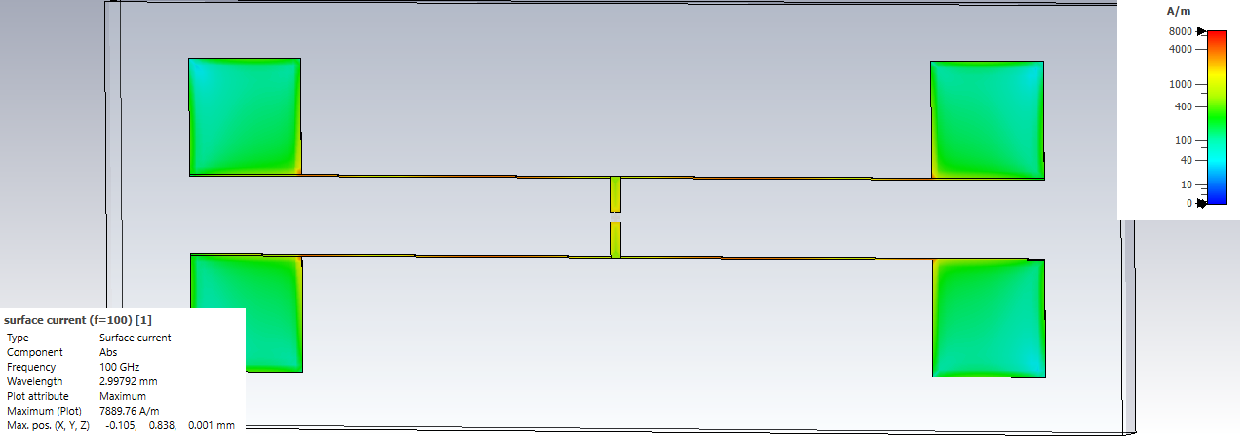
\includegraphics[width=\textwidth]{figures/contour_plots/Contour_ref_0.1THz_SC.pdf}
        \caption{}
        \label{contour_ref_100GHz}
    \end{subfigure}
    \hfill
    \begin{subfigure}[b]{1.1\textwidth}
        \centering
        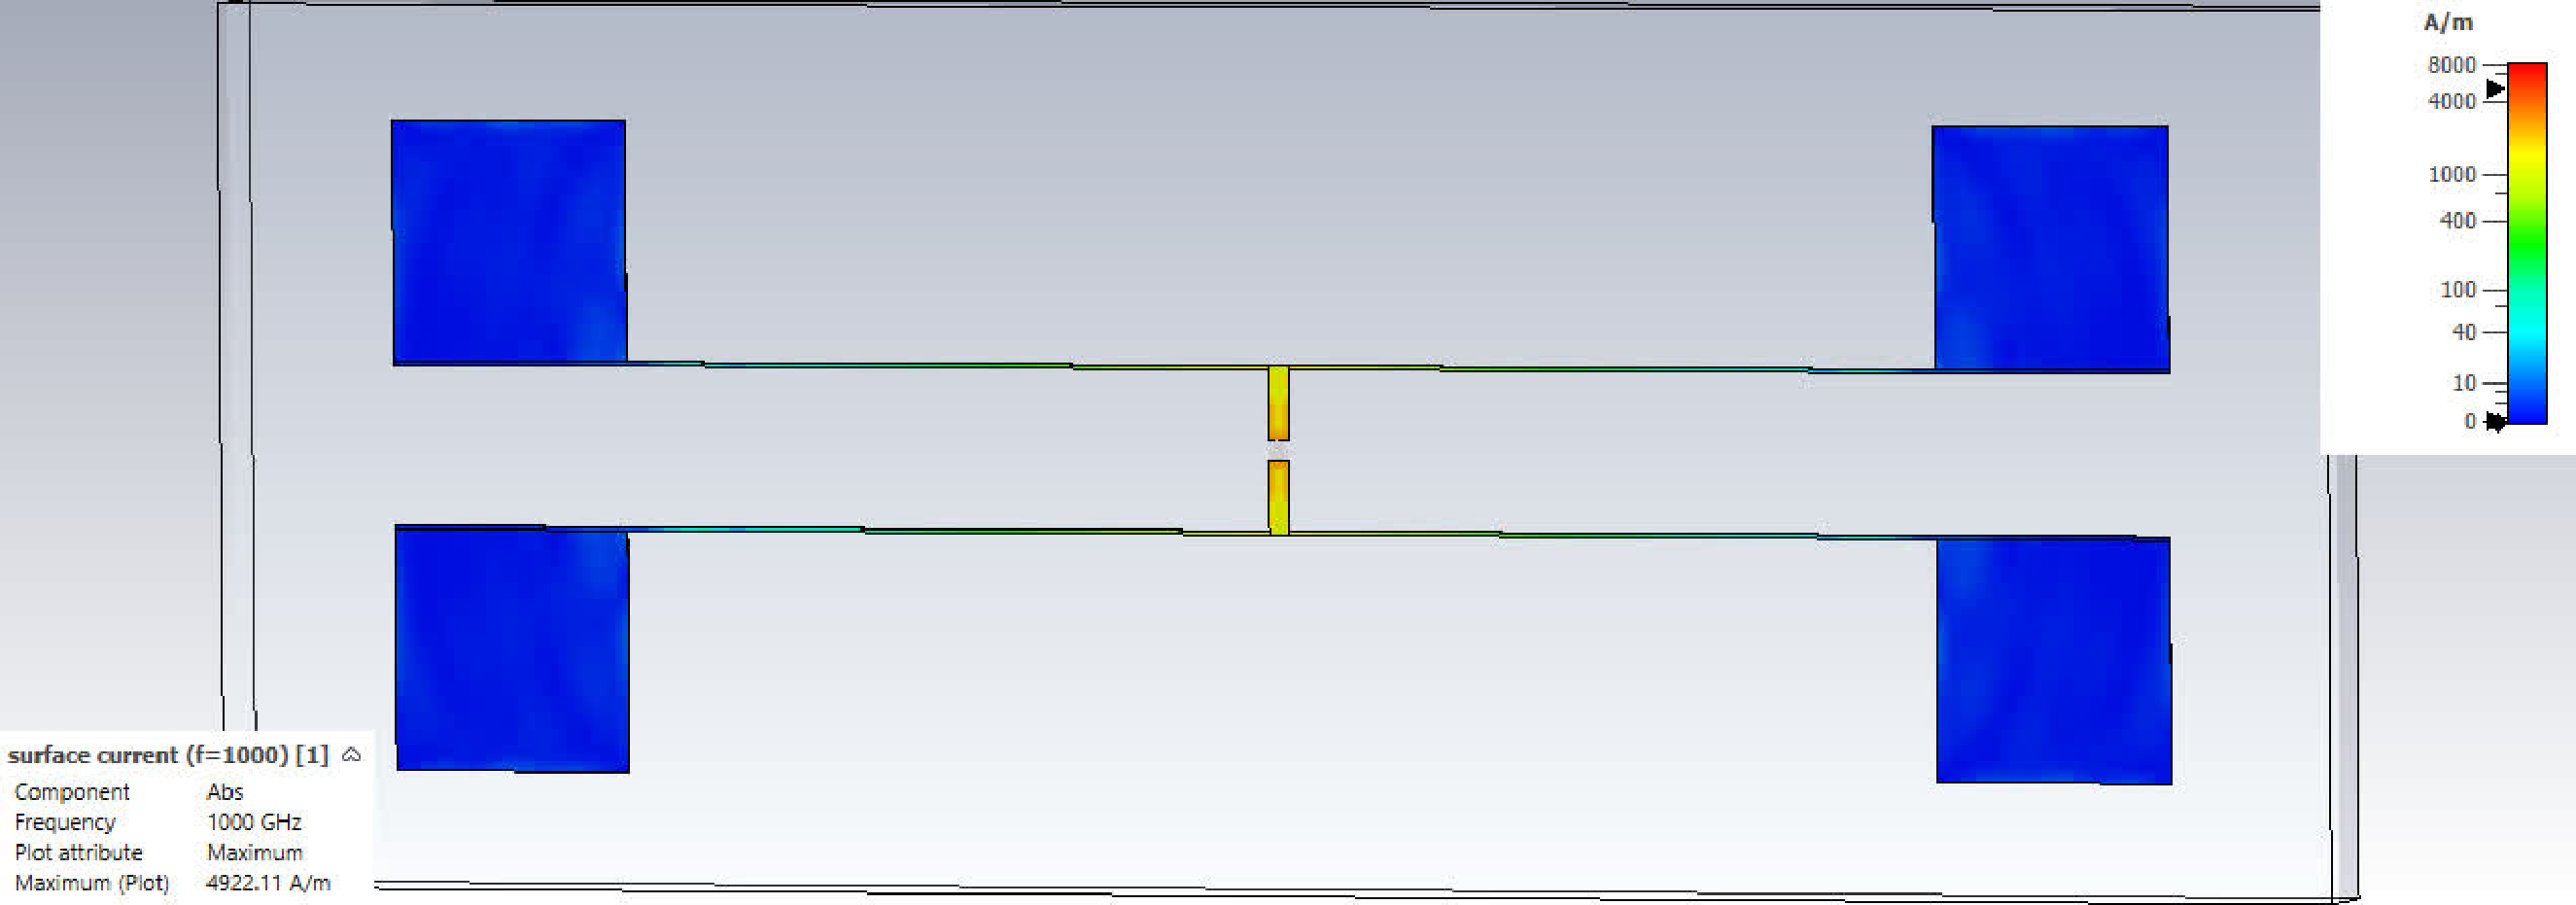
\includegraphics[width=\textwidth]{figures/contour_plots/Contour_ref_1THz_SC.pdf}
        \caption{}
        \label{contour_ref_1THz}
    \end{subfigure}
    \caption{Different PCAs and their general electrode structures are illustrated. Each antenna is designed with rectangular pads for probing. (a) Dimensions of H-Dipole electrodes. (b) Dimensions of bow-tie electrodes. (c) Dimensions of slotline antenna.}
    \label{electrodes_main}
\end{figure}



\chapter{Device Fabrication and DC Characterization}
\section{Device Fabrication Process}
\section{DC Characterization ??}

\chapter{Experimental Setup}
\section{THz TDS setup}
\section{Alignment ??}
\section{Data Analysis ??}

\chapter{Results and Discussion}

\chapter{Summary and Outlook}

\printbibliography

\end{document}
